\sectionthree{Characteristic equation: homogeneous case}
\begin{python0}
from solutions import *; clear() 
\end{python0}

Now that you're an expert on generating functions and 
recurrences, let's step back and look at our computations again.
For instance you notice that in many of the computations,
it seems like there's a pattern.

Suppose we go back to the original homogeneous degree 2 case:
\begin{align*}
a_n = c_1 a_{n-1} + c_2 a_{n-2}
\end{align*}
Then if we let $a(x) = \sum_{n=0}^\infty a_n x^n$, then
\begin{align*}
a(x) 
&= a_0 + a_1x + \sum_{n=2}^\infty a_n x^n \\
&= a_0 + a_1x + \sum_{n=2}^\infty (c_1 a_{n-1} + c_2 a_{n-2}) x^n \\
&= a_0 + a_1x + c_1 x(-a_0 + a(x)) + c_2 x^2 a(x) \\
\therefore\,\,\,\,\,
a(x) &= 
\frac{a_0 + (a_1 - c_1a_0)x}{1 - c_1x - c_2x^2}
\end{align*}

Now if you step back and look at the above, you see that the next step
is determined by the factorization of $1 - c_1x - c_2x^2$ and furthermore
that if the roots of $c_2x^2 + c_1 x - 1$ factorization is say
\[
(x - r_1)(x - r_2)
\]
with $r_1 \neq r_2$, then the rational function for $a(x)$ has the
form
\begin{align*}
a(x) 
& = (A + Bx)\biggl( \frac{C}{x - r_1} + \frac{D}{x - r_2} \biggr ) 
\end{align*}
which would lead to
\begin{align*}
a(x) 
& = (A + Bx)\biggl( 
\frac{-C}{r_1} \cdot \sum_{n=0}^\infty \frac{1}{r_1^n}x^n 
+
\frac{-D}{r_2} \cdot \sum_{n=0}^\infty \frac{1}{r_2^n}x^n 
\biggr) 
\end{align*}
which implies that $a(x)$ has the following form:
\begin{align*}
a(x) 
& = (A + Bx)\biggl( 
E \cdot \sum_{n=0}^\infty \frac{1}{r_1^n}x^n 
+
F \cdot \sum_{n=0}^\infty \frac{1}{r_2^n}x^n 
\biggr) 
\end{align*}
and if we stare harder:
\begin{align*}
a(x) 
&=  
AE \cdot \sum_{n=0}^\infty \frac{1}{r_1^n}x^n +
BF \cdot \sum_{n=0}^\infty \frac{1}{r_1^n}x^{n+1}
\\ 
&\hskip 0.5cm
+
AE \cdot \sum_{n=0}^\infty \frac{1}{r_2^n}x^n +
BE \cdot \sum_{n=0}^\infty \frac{1}{r_2^n}x^{n+1} \\
&=  
AE + 
\sum_{n=1}^\infty \frac{AE + BEr_1}{r_1^n} x^n +
\\ 
&\hskip 0.5cm
+
AF + 
\sum_{n=1}^\infty \frac{AF + BFr_2}{r_2^n} x^n\\
&=  
-BEr_1 + \frac{AE + BEr_1}{r_1^0} +
\sum_{n=1}^\infty \frac{AE + BEr_1}{r_1^n} x^n +
\\ 
&\hskip 0.5cm
+
-BFr_2 + \frac{AF + BFr_2}{r_2^0} +
\sum_{n=1}^\infty \frac{AF + BFr_2}{r_2^n} x^n \\
&=  
-BEr_1 + 
\sum_{n=0}^\infty \frac{AE + BEr_1}{r_1^n} x^n
\\ 
&\hskip 0.5cm
-BFr_2 +
\sum_{n=0}^\infty \frac{AF + BFr_2}{r_2^n} x^n
\end{align*}
Now let's look at 
\[
-BE r_1 - BFr_2
\]
If you go back a couple of steps you will see that
\[
E = \frac{-C}{r_1}, \,\,\,\,\, 
F = \frac{-D}{r_2}
\]
Therefore
\[
Er_1 + Fr_2 = -C-D
\]
and that $C$ and $D$ are constants such that
\[
\frac{1}{(x-r_1)(x - r_2)} = \frac{C}{x - r_1} + \frac{D}{x - r_2}
\]
From the partial fraction decomposition we get
\[
1 = C(x - r_2) + D(x - r_1) = (C+D)x + (-Cr_2 -Dr_1) 
\]
By the comparing the coefficients on both sides of this identity we see that
\[
C + D = 0
\]
Hence
\[
Er_1 + Fr_2 = -C-D = 0
\]
Amazing!
This means that
\begin{align*}
a(x) 
=
\sum_{n=0}^\infty \frac{AE + BEr_1}{r_1^n} x^n 
+
\sum_{n=0}^\infty \frac{AF + BFr_2}{r_2^n} x^n
\end{align*}

Now you might say: so what? The coefficients for $x^n$
still have to be determined ...
and the above doesn't simplify the process since we still have to 
compute the constants $A, B, E, F$, etc ... blah, blah, blah.

But wait! Hang on there!

The above shows that
\[
a(x) = 
\sum_{n=0}^\infty \frac{C_1}{r_1^n} x^n + 
\sum_{n=0}^\infty \frac{C_2}{r_2^n} x^n
\]
where $C_1, C_2$ are constants and $r_1, r_2$
are roots of $1 - c_1 x - c_2 x^2$. 
The computation of $r_1$ and $r_2$ is unavoidable.
In any case that's just an application of the quadratic equation formula.
How hard is that?

What about $C_1$ and $C_2$? 
Does the above form of $a(x)$ simplify the computation of $C_1$ 
and $C_2$? 
Well from
\[
a(x) = 
\sum_{n=0}^\infty \frac{C_1}{r_1^n} x^n + 
\sum_{n=0}^\infty \frac{C_2}{r_2^n} x^n
\]
we know that
\[
a_n = C_1 \frac{1}{r_1^n} + C_2 \frac{1}{r_1^n}
\]
Well we can use the values of $a_0$ and $a_1$ (or any two values
from the sequence of $a_n$ that we know) and get two linear
equations:
\begin{align*}
a_0 &= C_1  + C_2 \\
a_1 &= \frac{1}{r_1} \cdot C_1 + \frac{1}{r_2} \cdot C_2
\end{align*}
and then solve for $C_1$ and $C_2$.
This is just solving a system of two linear equations.
No big deal.

So let's summarize what we know:
Suppose we have the following homogeneous degree 2 recurrence relation:
\[
a_n = c_1 a_{n-1} + c_2 a_{n-2}
\]
then 
\begin{enumerate}
\item[$\bullet$] First we find the roots of $1 - c_1x - c_2x^2$. 
Say the roots $r_1$, $r_2$ are distinct.
\item[$\bullet$] Then we know that there are constants such that
\[
a_n = C_1 \frac{1}{r_1^n} + C_2 \frac{1}{r^n_2}
\]
\item[$\bullet$] We substitute two values of $n$ into the above closed
form for $a_n$ to get two linear equations for $C_1$ and $C_2$ and
solve for these constants.
\end{enumerate}

Note that for $r = r_1$ or $r_2$:
\[
1 - c_1 r - c_2 r^2 = 0
\]
And if we multiply this equation by $1/r^2$ we get
\[
\biggl( \frac{1}{r} \biggr)^2 - c_1 \biggl( \frac{1}{r}\biggr) - c_2 = 0
\]
Therefore if we look at this equation
\[
x^2 - c_1x - c_2 = 0
\]
the roots we get are reciprocals of our original $r_1$ and $r_2$, i.e.
if we let $s_1, s_2$ be roots 
\[
x^2 - c_1x - c_2 = 0
\] 
then $s_1 = 1/r_1, s_2 = 1/r_2$.
And with these roots instead of writing
\[
a_n = C_1 \frac{1}{r_1^n} + C_2 \frac{1}{r^n_2}
\]
we write
\[
a_n = C_1 {s_1^n} + C_2 {s^n_2}
\]

In summary:
If we're given this recurrence relation:
\[
a_n = c_1 a_{n-1} + c_2 a_{n-2}
\]
then we do the following:

Assume $a_n = s^n$ is a solution where $s \in \R$, i.e.,
\[
s^n = c_1 s^{n-1} + c_2 s^{n-2}
\]
Crossing out $s^{n-2}$, the above equation becomes
the following quadratic equation in $s$:
\[
s^2 = c_1 s + c_2
\]
i.e.,
\[
s^2 - c_1 s - c_2 = 0
\]
Find roots $s_1, s_2$ of the quadratic equation
\[
x^2 - c_1 x - c_2 = 0
\]

\begin{enumerate}[nosep]
\li 
Suppose $s_1 \neq s_2$.
Then the general closed form of $a_n$ must be
\[
a_n = C_1 s_1^n + C_2 s_2^n
\]
for some constants $C_1$ and $C_2$.
\li
Suppose $s_1 \neq s_2$.
Then the general closed form of $a_n$ must be
\[
a_n = C_1 s_1^n + C_2 ns_2^n
\]
for some constants $C_1$ and $C_2$.
\end{enumerate}
In both cases, to compute $C_1$ and $C_2$, substitute two values
for $n$ in the above closed form and solve for $C_1$ and $C_2$. 

The quadratic equation
\[
x^2 - c_1 x - c_2 = 0
\]
is called the
\defone{characteristic equation} of the recurrence relation.


Let's use the above method to find the closed form for 
the Fibonacci sequence
\[
F_n = \begin{cases}
0 &\text{ if } n = 0 \\
1 &\text{ if } n = 1 \\
F_{n-1} + F_{n-2} &\text{ if } n \geq 2
\end{cases}
\]
The recurrence relation is
\[
F_n = F_{n - 1} + F_{n-2}
\]
i.e.
\[
F_n - F_{n - 1} - F_{n-2} = 0
\]
The quadratic equation to solve is
\[
x^2 - x - 1 = 0
\]
The roots are
\[
\frac{1 + \sqrt{5}}{2}, \,\,\,\,\,
\frac{1 - \sqrt{5}}{2}
\]
Hence the closed form must be 
\[
F_n = C_1 \biggl( \frac{1 + \sqrt{5}}{2} \biggr)^n
+ C_2 \biggl( \frac{1 - \sqrt{5}}{2} \biggr)^n
\]
To solve for $C_1$ and $C_2$, let $n = 0, 1$ and we get
\begin{align*}
0 &= F_0 = C_1 + C_2 \\
1 &= F_1 = C_1 \frac{1 + \sqrt{5}}{2} + C_2 \frac{1 - \sqrt{5}}{2}
\end{align*}
The first equation implies that $C_2 = - C_1$ and hence we get
\begin{align*}
1 &= C_1 \frac{1 + \sqrt{5}}{2} - C_1 \frac{1 - \sqrt{5}}{2} \\
\therefore \,\,\,\,\, 
1 &= C_1 \sqrt{5} \\
\therefore\,\,\,\,\,
C_1 &= \frac{1}{\sqrt{5}}
\end{align*}
Therefore $C_2 = -\frac{1}{\sqrt{5}}$. 
Hence
\[
F_n = 
\frac{1}{\sqrt{5}} \biggl( \frac{1 + \sqrt{5}}{2} \biggr)^n
-
\frac{1}{\sqrt{5}}
\biggl( \frac{1 - \sqrt{5}}{2} \biggr)^n
\]
which we already know from a previous section.

Note that the whole point of this computational technique is to 
\textit{delay} the computation of certain constants until after we have
a closed form for our sequence.
The closed form has unknown constants (made up of constants
which were left unresolved).
Finally the constants in the closed form are resolved by writing
down linear equations for the constants using
known values from the sequence.

\begin{eg}
  Consider the homogeneous degree 2 linear recurrence
  \[
  a_n = 5a_{n-1} - 6a_{n-2}
  \]
  \begin{enumerate}[nosep,label=(\alph*)]
  \item What is the characteristic equation?
  \item What are the roots of the characteristic equation?
  \item What is the general closed form for $a_n$?
  \item If $a_0 = 1, a_1 = 3$, what is the closed form for $a_n$?
  \end{enumerate}
\end{eg}
\SOLUTION
(a) Let $a_n = r^n$ be a solution of the recurrence relation.
Then
\[
r^n = 5 r^{n-1} - 6 r^{n-2}
\]
Hence
\[
r^2 - 5 r + 6 = 0
\]
Therefore the characteristic equation of the recurrence relation
is
\[
x^2 - 5x + 6 = 0
\]
(b)
Using the qudratic equation formula,
the roots of the characteristic equation from (a) are
\[
r = \frac{5 \pm \sqrt{5^2 - 4 \cdot 1 \cdot 6}}{2} = 2, 3
\]
(c)
The general closed form for $a_n$ is
\[
a_n = C_1 2^n + C_2 3^n
\]
(d)
From $a_0 = 1, a_1 = 3$, we have
\begin{align*}
  1 &= a_0 = C_1 + C_2 \\
  3 &= a_1 = 2C_1 + 3C_2 
\end{align*}
Hence $C_1 = 0, C_2 = 1$.
Therefore
\[
a_n = 3^n
\]
for $n \geq 0$.

(Check: $3^0 = 1 = a_0$, $3^1 = 3 = a_1$. So $3^n$ matches
the two base cases.
For $n = 2$,
$3^2 = 9$ and $a_2 = 5a_{1} - 6a_{0} = 5 \cdot 3 - 6 \cdot 1 = 9$.)
\qed


\begin{ex} 
  \label{ex:some-decision1}
  \tinysidebar{\debug{exercises/{empty0/question.tex}}}
  \solutionlink{sol:some-decision1}
  \qed
\end{ex} 
\begin{python0}
from solutions import *
add(label="ex:some-decision1",
    srcfilename='exercises/some-decision1/answer.tex') 
\end{python0}


In general if you are given a
homogeneous linear recurrence relation of degree $d$:
\[
a_n = c_1 a_{n-1} + c_2 a_{n-2} + \cdots + c_d a_{n - d}
\]
it can be shown that the following works:
Find all the roots of 
\[
x^d - c_1 x^{d-1} - c_2 x^{d-2} - \cdots - c_d = 0
\]
\begin{enumerate}[nosep]
\li Suppose the roots $r_1, \ldots, r_d$ are distinct.
Then there are constants $C_1, \ldots, C_d$
such that
\[
a_n = C_1 r_1^n + C_2 r_2^n + \cdots + C_d r_d^n
\]
\li
Now suppose some roots repeat.
Suppose $r_1$ appear exactly $5$ times in the factorization of the
characteristic equation, then the part of the closed form of $a_n$ 
that involves $r_1$ will contain a linear combination of
the following 5 terms:
$r_1^n$, $nr_1^n$, $n^2 r_1^n, n^3r_1^n, n^{4} r_1^n$.
In other words $a_n$ will look like this:
\[
a_n = 
\biggl( 
C_1 r_1^n + C_2nr_1^n + C_3n^2r_1^n + C_4n^3r_1^n + C_5 n^{4}r_1^n
\biggr)
+ \cdots
\]
where $C_1, ..., C_5$ are constants.
Now suppose root $r_2$, which is different from $r_1$,
appears 3 times.
Then
\begin{align*}
  a_n
  &= 
  \biggl( 
  C_1 r_1^n + C_2nr_1^n + C_3n^2r_1^n + C_4n^3r_1^n + C_5 n^{4}r_1^n
  \biggr)
  \\
  &\hspace{1cm} +
  \biggl( 
  C_6 r_2^n + C_7nr_2^n + C_8n^2r_2^n 
  \biggr)
  + \cdots
\end{align*}
where $C_1, ..., C_8$ are constants.
Now suppose root $r_3$, which is different from $r_1$ and $r_2$,
appears 2 times.
Then
\begin{align*}
  a_n
  &= 
  \biggl( 
  C_1 r_1^n + C_2nr_1^n + C_3n^2r_1^n + C_4n^3r_1^n + C_5 n^{4}r_1^n
  \biggr)
  \\
  &\hspace{1cm} +
  \biggl( 
  C_6 r_2^n + C_7nr_2^n + C_8n^2r_2^n 
  \biggr)
  \\
  &\hspace{1cm} +
  \biggl( 
  C_9 r_3^n + C_{10}nr_3^n 
  \biggr)
  + \cdots
\end{align*}
where $C_1, ..., C_{10}$ are constants.
And you keep going until all roots are accounted for.
\end{enumerate}

[Aside: Those of you who took Diff Eq, why does this feel like
de jevu? Check your notes on homogeneous differential equations.]


For instance suppose that the characteristic equation looks like this:
\[
\biggl( x - \frac{1}{2} \biggr)
\biggl( x - \frac{1}{3} \biggr)
\biggl( x - \frac{5}{7} \biggr)^4
\biggl( x - \frac{2}{13} \biggr)^2
= 0
\]
Then we must have
\begin{align*}
a_n &= 
A \biggl( \frac{1}{2} \biggr)^n \\
&\hskip 0.5cm 
+ B \biggl( \frac{1}{3} \biggr)^n \\
&\hskip 0.5cm 
+ C \biggl( \frac{5}{7} \biggr)^n +
D n\biggl( \frac{5}{7} \biggr)^n +
E n^2\biggl( \frac{5}{7} \biggr)^n +
F n^3\biggl( \frac{5}{7} \biggr)^n \\
&\hskip 0.5cm 
+ G \biggl( \frac{2}{13} \biggr)^n +
H n\biggl( \frac{2}{13} \biggr)^n
\end{align*}

[EXERCISES]

\textsc{Aside}.

Why is the quadratic equation of a degree 2 recurrence relation
called the characteristic equation?
And if you've taken linear algebra you should be scratching your
head and asking yourself why does this sounds so familiar.

I've already mentioned that you can view $\sum_{n=0}^\infty a_n x^n$
as an infinite dimensional vector:
\[
(a_0, a_1, a_2, \ldots)
\]
Recall that multiplication by $x^\ell$ acts as a shift-by-$\ell$ operator
on $\sum_{n=0}^\infty a_n x^n$.
Let me write $T$ for \textit{left} shift operator.
\[
T((a_0, a_1, a_2, \ldots)) = (a_1, a_2, a_3, \ldots)
\]
The corresponding action on a power series is
\[
\sum_{n=0}^\infty a_n x^n \rightarrow \frac{\sum_{n=0}^\infty a_n x^n - a_0}{x}
\]
Let $T^n$ be applying $T$ $n$ times, i.e., the left-shift-by-$n$ operator.
Suppose we look at the case of Fibonacci sequence:
\[
F_n = F_{n-1} + F_{n-2}
\]
Then I have the following:
\begin{align*}
T^2((F_0, F_1, F_2, \ldots)) &= (F_2, F_3, F_4, \ldots) \\
T^1((F_0, F_1, F_2, \ldots)) &= (F_1, F_2, F_3, \ldots) \\
T^0((F_0, F_1, F_2, \ldots)) &= (F_0, F_1, F_2, \ldots)
\end{align*}
and therefore
\begin{align*}
(T^2 - T^1 - T^0)((F_0, F_1, F_2, \ldots)) 
&= (F_2 - F_1 - F_0, F_3 - F_2 - F_1, F_4 - F_3 - F_2, \ldots)
\end{align*}
Since $F_n = F_{n-1} + F_{n-2}$ for $n \geq 2$, the above is in fact
\begin{align*}
(T^2 - T^1 - T^0)((F_0, F_1, F_2, \ldots)) 
&= (0, 0, 0, \ldots)
\end{align*}
In other words the $T^2 - T^1 - T^0$ acts like the multiplication by $0$
operator on $(F_0, F_1, F_2, \ldots)$:
\[
T^2 - T^1 - T^0 = 0
\]
The corresponding polynomial 
\[
x^2 - x - 1
\]
is called the characteristic polynomial of $T$.

\newpage
\subsection*{Solutions}

\newpage
\section*{Solutions}
Solution to Exercise \ref{ex:dfa0}\labeltext{}{sol:dfa0}.

\tinysidebar{\debug{exercises/{dfa0/answer.tex}}}

    Solution not provided.
    

\newpage

Solution to Exercise \ref{ex:dfa1}\labeltext{}{sol:dfa1}.

\tinysidebar{\debug{exercises/{dfa1/answer.tex}}}
  The ID computation is
  \begin{align*}
    (q_0, aba)
    &\vdash (\delta(q_0, a), ba) = (q_0, ba) \\ 
    &\vdash (\delta(q_0, b), a) = (q_1, a) \\
    &\vdash (\delta(q_1, a), \ep) = (q_0, \ep)
  \end{align*}
  $q_0$ is not an accept state. Therefore $aba$ is not accepted.


\newpage

Solution to Exercise \ref{ex:dfa4}\labeltext{}{sol:dfa4}.

\tinysidebar{\debug{exercises/{dfa4/answer.tex}}}

    Solution not provided.
    

\newpage

Solution to Exercise \ref{ex:dfa5}\labeltext{}{sol:dfa5}.

\tinysidebar{\debug{exercises/{dfa5/answer.tex}}}

    Solution not provided.
    

\newpage

Solution to Exercise \ref{ex:implementing-a-single-dfa0}\labeltext{}{sol:implementing-a-single-dfa0}.

\tinysidebar{\debug{exercises/{implementing-a-single-dfa0/answer.tex}}}

    Solution not provided.
    

\newpage

Solution to Exercise \ref{ex:nfastatediag0}\labeltext{}{sol:nfastatediag0}.

\tinysidebar{\debug{exercises/{nfastatediag0/answer.tex}}}

    Solution not provided.
    

\newpage

Solution to Exercise \ref{ex:nfastatediag1}\labeltext{}{sol:nfastatediag1}.

\tinysidebar{\debug{exercises/{nfastatediag1/answer.tex}}}

    Solution not provided.
    

\newpage

Solution to Exercise \ref{ex:nfastatediag2}\labeltext{}{sol:nfastatediag2}.

\tinysidebar{\debug{exercises/{nfastatediag2/answer.tex}}}

    Solution not provided.
    

\newpage

Solution to Exercise \ref{ex:nfastatediag3}\labeltext{}{sol:nfastatediag3}.

\tinysidebar{\debug{exercises/{nfastatediag3/answer.tex}}}

    Solution not provided.
    

\newpage

Solution to Exercise \ref{ex:nfastatediag4}\labeltext{}{sol:nfastatediag4}.

\tinysidebar{\debug{exercises/{nfastatediag4/answer.tex}}}

    Solution not provided.
    

\newpage

Solution to Exercise \ref{ex:nfastatediag5}\labeltext{}{sol:nfastatediag5}.

\tinysidebar{\debug{exercises/{nfastatediag5/answer.tex}}}

    Solution not provided.
    

\newpage

Solution to Exercise \ref{ex:nfastatediag6}\labeltext{}{sol:nfastatediag6}.

\tinysidebar{\debug{exercises/{nfastatediag6/answer.tex}}}

    Solution not provided.
    

\newpage

Solution to Exercise \ref{ex:nfastatediag7}\labeltext{}{sol:nfastatediag7}.

\tinysidebar{\debug{exercises/{nfastatediag7/answer.tex}}}

    Solution not provided.
    

\newpage

Solution to Exercise \ref{ex:nfastatediag8}\labeltext{}{sol:nfastatediag8}.

\tinysidebar{\debug{exercises/{nfastatediag8/answer.tex}}}

    Solution not provided.
    

\newpage

Solution to Exercise \ref{ex:nfastatediag9}\labeltext{}{sol:nfastatediag9}.

\tinysidebar{\debug{exercises/{nfastatediag9/answer.tex}}}

    Solution not provided.
    

\newpage

Solution to Exercise \ref{ex:nfastatediag10}\labeltext{}{sol:nfastatediag10}.

\tinysidebar{\debug{exercises/{nfastatediag10/answer.tex}}}

    Solution not provided.
    

\newpage

Solution to Exercise \ref{ex:nfastatediag11}\labeltext{}{sol:nfastatediag11}.

\tinysidebar{\debug{exercises/{nfastatediag11/answer.tex}}}

    Solution not provided.
    

\newpage

Solution to Exercise \ref{ex:nfastatediag12}\labeltext{}{sol:nfastatediag12}.

\tinysidebar{\debug{exercises/{nfastatediag12/answer.tex}}}

    Solution not provided.
    

\newpage

Solution to Exercise \ref{ex:nfastatediag13}\labeltext{}{sol:nfastatediag13}.

\tinysidebar{\debug{exercises/{nfastatediag13/answer.tex}}}

    Solution not provided.
    

\newpage

Solution to Exercise \ref{ex:nfa0}\labeltext{}{sol:nfa0}.

\tinysidebar{\debug{exercises/{nfa0/answer.tex}}}
The formal definition of this NFA is $(\Sigma, Q, q_0, \delta, F)$ where
\begin{tightlist}
\li $\Sigma = \{a,b\}$
\li $Q = \{q_0\}$
\li $\delta$ is the function
\[
\delta : Q \times \Sigma_\epsilon \rightarrow P(Q)
\]
given by
\begin{align*}
  \delta(q_0, \epsilon) &= \{\} \\
  \delta(q_0, a) &= \{\} \\
  \delta(q_0, b) &= \{\} 
\end{align*}
\end{tightlist}


\newpage

Solution to Exercise \ref{ex:nfa1}\labeltext{}{sol:nfa1}.

\tinysidebar{\debug{exercises/{nfa1/answer.tex}}}

    Solution not provided.
    

\newpage

Solution to Exercise \ref{ex:nfa2}\labeltext{}{sol:nfa2}.

\tinysidebar{\debug{exercises/{nfa2/answer.tex}}}

    Solution not provided.
    

\newpage

Solution to Exercise \ref{ex:nfa3}\labeltext{}{sol:nfa3}.

\tinysidebar{\debug{exercises/{nfa3/answer.tex}}}

    Solution not provided.
    

\newpage

Solution to Exercise \ref{ex:nfa4}\labeltext{}{sol:nfa4}.

\tinysidebar{\debug{exercises/{nfa4/answer.tex}}}

    Solution not provided.
    

\newpage

Solution to Exercise \ref{ex:nfa5}\labeltext{}{sol:nfa5}.

\tinysidebar{\debug{exercises/{nfa5/answer.tex}}}

    Solution not provided.
    

\newpage

Solution to Exercise \ref{ex:dfa-as-powerful-as-nfa0}\labeltext{}{sol:dfa-as-powerful-as-nfa0}.

\tinysidebar{\debug{exercises/{dfa-as-powerful-as-nfa0/answer.tex}}}
Here's the solution.
Let $\delta$ denote the transition function of $N$.
Note that 
\begin{align*}
  \delta(q_0, \epsilon) = \{\} \\
  \delta(q_0, a) = \{\} \\
  \delta(q_0, b) = \{\} 
\end{align*}
First of all the states are labeled as all the subsets of $\{q_0\}$.


\begin{center}
\begin{tikzpicture}[>=triangle 60,shorten >=0.5pt,node distance=2cm,auto,initial text=, double distance=2pt]
\node[state] (A) at (  0,  0) {$\{q_0\}$};
\node[state] (B) at (  3,  0) {$\{\}$};

\path[->]

;
\end{tikzpicture}
\end{center}
    


The start state is the $\epsilon$-closure of $\{q_0\}$.
However in $N$, there are no $\epsilon$--transitions out of 
$q_0$.
So the $\epsilon$-closure of $\{q_0\}$ is in fact $\{q_0\}$, i.e.
$\overline{\{q_0\}} = \{q_0\}$
The $\DFA$ is now this:


\begin{longtable}{|r||r|r|r|r|r|}
\hline 
         & $w_1$ & $w_2$ & $w_3$ & $w_4$ & $\ldots$ \\ \hline \hline 
$M_1$    &       &       &       &       &          \\ \hline 
$M_2$    &       &       &       &       &          \\ \hline 
$M_3$    &       &       &       &       &          \\ \hline 
$M_4$    &       &       &       &       &          \\ \hline 
$\ldots$ &       &       &       &       &          \\ \hline 
\end{longtable}
        


Now I will compute the $a$--transition of the state $\{q_0\}$.
Let $\delta^\DFA$ denote the transition function of the $\DFA$
that we're building.
Then
\begin{align*}
\delta( \{q_0, a\} ) 
&= \overline{ \bigcup_{q \in \{q_0\}} \delta(q, a)} \\
&= \overline{ \delta(q_0, a) } \\
&= \overline{ \emptyset } \\
&= \emptyset
\end{align*}
The (incomplete) $\DFA$ now looks like this:


\begin{longtable}{|r||r|r|r|r|r|}
\hline 
         & $w_1$ & $w_2$ & $w_3$ & $w_4$ & $\ldots$ \\ \hline \hline 
$M_1$    & 0     & 0     & 1     & 0     & ...      \\ \hline 
$M_2$    & 1     & 0     & 1     & 1     & ...      \\ \hline 
$M_3$    & 0     & 1     & 1     & 1     & ...      \\ \hline 
$M_4$    & 1     & 0     & 1     & 1     & ...      \\ \hline 
$\ldots$ &       &       &       &       &          \\ \hline 
\end{longtable}
        


Using the same reasoning we have

\begin{center}
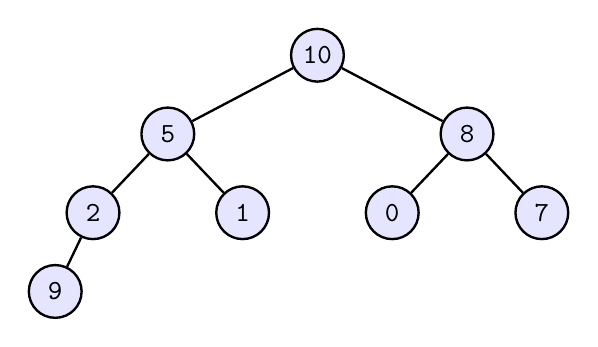
\begin{tikzpicture}

\fill[blue!10] (0.0, 0.0) circle (0.35);
\node [line width=0.03cm,black,minimum size=0.6699999999999999cm,draw,circle] at (0.0,0.0)(10){};\draw (0.0, 0.0) node[color=black] {\texttt{10}};
\fill[blue!10] (-1.9, -1.0) circle (0.35);
\node [line width=0.03cm,black,minimum size=0.6699999999999999cm,draw,circle] at (-1.9,-1.0)(5){};\draw (-1.9, -1.0) node[color=black] {\texttt{5}};
\fill[blue!10] (1.9, -1.0) circle (0.35);
\node [line width=0.03cm,black,minimum size=0.6699999999999999cm,draw,circle] at (1.9,-1.0)(8){};\draw (1.9, -1.0) node[color=black] {\texttt{8}};
\fill[blue!10] (-2.85, -2.0) circle (0.35);
\node [line width=0.03cm,black,minimum size=0.6699999999999999cm,draw,circle] at (-2.85,-2.0)(2){};\draw (-2.85, -2.0) node[color=black] {\texttt{2}};
\fill[blue!10] (-0.95, -2.0) circle (0.35);
\node [line width=0.03cm,black,minimum size=0.6699999999999999cm,draw,circle] at (-0.95,-2.0)(1){};\draw (-0.95, -2.0) node[color=black] {\texttt{1}};
\fill[blue!10] (0.95, -2.0) circle (0.35);
\node [line width=0.03cm,black,minimum size=0.6699999999999999cm,draw,circle] at (0.95,-2.0)(0){};\draw (0.95, -2.0) node[color=black] {\texttt{0}};
\fill[blue!10] (2.85, -2.0) circle (0.35);
\node [line width=0.03cm,black,minimum size=0.6699999999999999cm,draw,circle] at (2.85,-2.0)(7){};\draw (2.85, -2.0) node[color=black] {\texttt{7}};
\fill[blue!10] (-3.33, -3.0) circle (0.35);
\node [line width=0.03cm,black,minimum size=0.6699999999999999cm,draw,circle] at (-3.33,-3.0)(9){};\draw (-3.33, -3.0) node[color=black] {\texttt{9}};\draw[line width=0.03cm,black] (10) to  (5);
\draw[line width=0.03cm,black] (10) to  (8);
\draw[line width=0.03cm,black] (5) to  (2);
\draw[line width=0.03cm,black] (5) to  (1);
\draw[line width=0.03cm,black] (8) to  (0);
\draw[line width=0.03cm,black] (8) to  (7);
\draw[line width=0.03cm,black] (2) to  (9);
\end{tikzpicture}

\end{center}



It's easy to see that in the DFA, the $a$--
and $b$--transitions from the state $\{\}$ goes back to itself.
Therefore the completed DFA is this:


\begin{center}
\begin{tikzpicture}[>=triangle 60,shorten >=0.5pt,node distance=2cm,auto,initial text=, double distance=2pt]
\node[state,initial] (A) at (  0,  0) {$\{q_0\}$};
\node[state] (B) at (  3,  0) {$\{\}$};

\path[->]
(A) edge [bend left=0,pos=0.5,above] node {$a,b$} (B)
(B) edge [loop above] node {$a,b$} ()

;
\end{tikzpicture}
\end{center}
    



\newpage

Solution to Exercise \ref{ex:dfa-as-powerful-as-nfa1}\labeltext{}{sol:dfa-as-powerful-as-nfa1}.

\tinysidebar{\debug{exercises/{dfa-as-powerful-as-nfa1/answer.tex}}}

    Solution not provided.
    

\newpage

Solution to Exercise \ref{ex:dfa-as-powerful-as-nfa2}\labeltext{}{sol:dfa-as-powerful-as-nfa2}.

\tinysidebar{\debug{exercises/{dfa-as-powerful-as-nfa2/answer.tex}}}

    Solution not provided.
    

\newpage

Solution to Exercise \ref{ex:dfa-as-powerful-as-nfa3}\labeltext{}{sol:dfa-as-powerful-as-nfa3}.

\tinysidebar{\debug{exercises/{dfa-as-powerful-as-nfa3/answer.tex}}}

    Solution not provided.
    

\newpage

Solution to Exercise \ref{ex:dfa-as-powerful-as-nfa4}\labeltext{}{sol:dfa-as-powerful-as-nfa4}.

\tinysidebar{\debug{exercises/{dfa-as-powerful-as-nfa4/answer.tex}}}

    Solution not provided.
    

\newpage

Solution to Exercise \ref{ex:closure0}\labeltext{}{sol:closure0}.

\tinysidebar{\debug{exercises/{closure0/answer.tex}}}

    Solution not provided.
    

\newpage

Solution to Exercise \ref{ex:closure1}\labeltext{}{sol:closure1}.

\tinysidebar{\debug{exercises/{closure1/answer.tex}}}

    Solution not provided.
    

\newpage

Solution to Exercise \ref{ex:closure2}\labeltext{}{sol:closure2}.

\tinysidebar{\debug{exercises/{closure2/answer.tex}}}

    Solution not provided.
    

\newpage

Solution to Exercise \ref{ex:closure3}\labeltext{}{sol:closure3}.

\tinysidebar{\debug{exercises/{closure3/answer.tex}}}

    Solution not provided.
    

\newpage

Solution to Exercise \ref{ex:closure4}\labeltext{}{sol:closure4}.

\tinysidebar{\debug{exercises/{closure4/answer.tex}}}

    Solution not provided.
    

\newpage

Solution to Exercise \ref{ex:closure5}\labeltext{}{sol:closure5}.

\tinysidebar{\debug{exercises/{closure5/answer.tex}}}

    Solution not provided.
    

\newpage

Solution to Exercise \ref{ex:closure6}\labeltext{}{sol:closure6}.

\tinysidebar{\debug{exercises/{closure6/answer.tex}}}

    Solution not provided.
    

\newpage

Solution to Exercise \ref{ex:closure7}\labeltext{}{sol:closure7}.

\tinysidebar{\debug{exercises/{closure7/answer.tex}}}

    Solution not provided.
    

\newpage

Solution to Exercise \ref{ex:closure8}\labeltext{}{sol:closure8}.

\tinysidebar{\debug{exercises/{closure8/answer.tex}}}

    Solution not provided.
    

\newpage

Solution to Exercise \ref{ex:closure9}\labeltext{}{sol:closure9}.

\tinysidebar{\debug{exercises/{closure9/answer.tex}}}

    Solution not provided.
    

\newpage

Solution to Exercise \ref{ex:closure10}\labeltext{}{sol:closure10}.

\tinysidebar{\debug{exercises/{closure10/answer.tex}}}

    Solution not provided.
    

\newpage

Solution to Exercise \ref{ex:closure11}\labeltext{}{sol:closure11}.

\tinysidebar{\debug{exercises/{closure11/answer.tex}}}

    Solution not provided.
    

\newpage

Solution to Exercise \ref{ex:closure12}\labeltext{}{sol:closure12}.

\tinysidebar{\debug{exercises/{closure12/answer.tex}}}

    Solution not provided.
    
 % input solutions.tex
